\label{lab:corrMvt}

\section{Introduction}

Nous allons maintenant présenter les techniques de correction du mouvement respiratoire présentées dans la littérature. 

Deux approches existent pour la correction du mouvement : les techniques dites prospectives, qui consistent à réaliser la correction pendant l'acquisition en sélectionnant les données à conserver, et rétrospectives, qui réalisent la correction à posteriori, après l'acquisition des données. Actuellement, les techniques les plus prometteuses sont rétrospectives, car elles permettent d'utiliser l'ensemble des données du cycle respiratoire.

\section{Synchronisation respiratoire}

La synchronisation respiratoire correspond à un découpage du cycle respiratoire selon la phase (voir Fig.\ref{fig:gatingRespi}) ou l'amplitude (voir figure \ref{fig:gatingRespiAmplitude}). Une seule des phases ou amplitude sera sélectionnée pour la reconstruction. En théorie cela permet d'avoir le meilleur résultat, car il est possible de sélectionner les évènements correspondants à la phase ou l'amplitude où a été acquise la carte d'atténuation.


\begin{figure}[h!]
	\begin{center}
		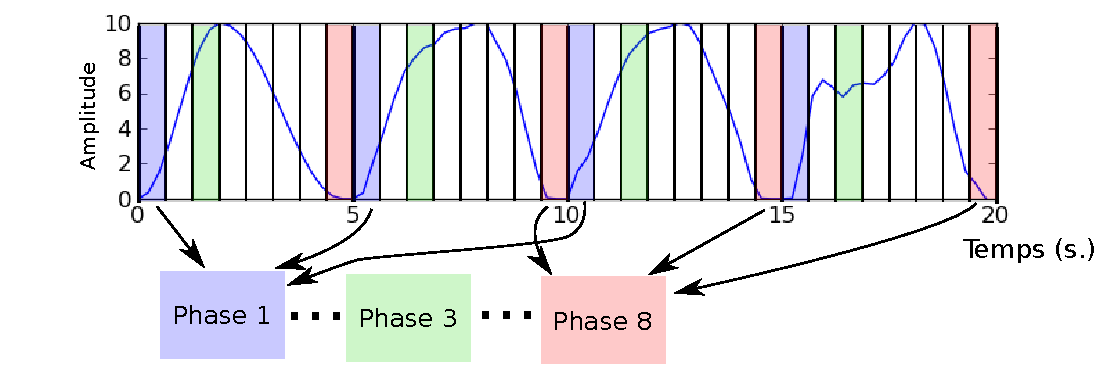
\includegraphics[width=12cm]{images/ET-IM}
	\end{center}
	\caption{Illustration de la synchronisation respiratoire en phase : Le cycle respiratoire acquis est découpé selon la position du signal acquis dans le cycle. Le signal est analysé pour déterminer les débuts et fins de cycles. Chaque cycle est découpé en un nombre déterminé de phases égales.} 
	\label{fig:gatingRespi}
\end{figure}


\begin{figure}[h!]
	\begin{center}
		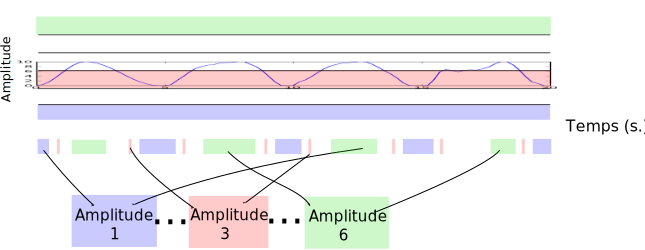
\includegraphics[width=12cm]{images/gatingAmplitude}
	\end{center}
	\caption{Illustration de la synchronisation respiratoire en amplitude : Le cycle respiratoire acquis est découpé selon son amplitude.} 
	\label{fig:gatingRespiAmplitude}
\end{figure}


Cette technique est notamment présentée dans~\cite{nehmeh2002effect}, où le signal respiratoire est estimé par une caméra qui suit un marqueur placé sur le torse du patient (système RPM de Varian Medical Systems). L'étude a été réalisée sur 5 patients volontaires comme suit : un scan de transmission de 3 minutes, suivi d'une acquisition avec correction de 10 minutes, puis d'une acquisition témoin non corrigée de 3 minutes. La décomposition du cycle s'effectue en fonction de la phase. L'auteur annonce une réduction du volume des tumeurs pouvant aller jusqu'à 34\%, avec une augmentation du $SUV_{max}$ de 160\%. 

Une autre publication~\cite{boucher2004respiratory} utilise un thermomètre détectant l'air chaud émis en début de cycle respiratoire pour réaliser la synchronisation. Les différentes reconstructions issues de l'expérience sont visibles figure \ref{fig:boucher2004}. Il faut noter que la partie clinique de cette étude a été réalisée sur 10 patients sains, et qu'il n'y a donc pas de mesures de performance de la correction du mouvement sur les lésions. 

\begin{figure}[h!]
	\begin{center}
		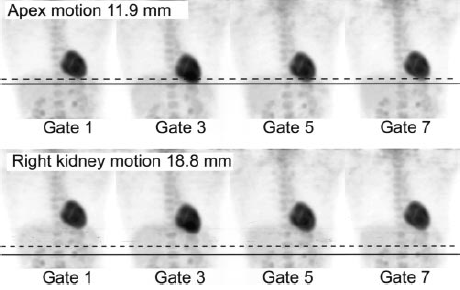
\includegraphics[width=12cm]{images/gatingBoucher2004}
	\end{center}
	\caption{Illustration de l'étendue du mouvement respiratoire sur des images reconstruites après synchronisation respiratoire~\cite{boucher2004respiratory}. La rangée du haut montre l'étendue du mouvement de l'apex du coeur, et celle du bas l'étendue du mouvement du rein} 
	\label{fig:boucher2004}
\end{figure}

Une variante de cette technique ne nécessitant pas de capteur est décrite dans~\cite{nehmeh2003reduction}. Un point faiblement radioactif est fixé au-dessus du torse du patient. Les acquisitions de l'imageur sont ensuite enregistrées par blocs temporels de 1 seconde, et une zone d'intérêt est reconstruite dans chacune des images. Les données reconstruites montrant le point source dans cette zone d'intérêt sont sommées et l'image finale reconstruite. 

Cette technique a été comparée avec celle présentée précédemment basée sur le système RPM. Ces deux techniques n'ont été testées cliniquement que sur un patient mais ont montrés des performances tout à fait semblables (6\% de différence dans les activités et 2\% pour le volume de la lésion).

Cependant ces techniques n'utilisent pas une carte d'atténuation optimisée pour la position du cycle correspondant aux acquisitions TEP.  Guoping et al.~\cite{GuopingChang2010Implementation} réalisent la carte d'atténuation à partir d'une image TDM réalisée en respiration libre synchronisée, et reconstruisent les données TEP acquises lorsque l'amplitude respiratoire est proche de celle utilisée pour l'acquisition TDM (voir exemples figure \ref{fig:chang2010}. Les résultats présentés sur 13 patients (21 tumeurs) montrent une amélioration du rapport signal sur bruit pouvant aller de -3.4 à 81\% suivant les tumeurs, avec une amélioration moyenne de 26.3\%.

\begin{figure}[h!]
	\begin{center}
		\begin{tabular}{c c}
			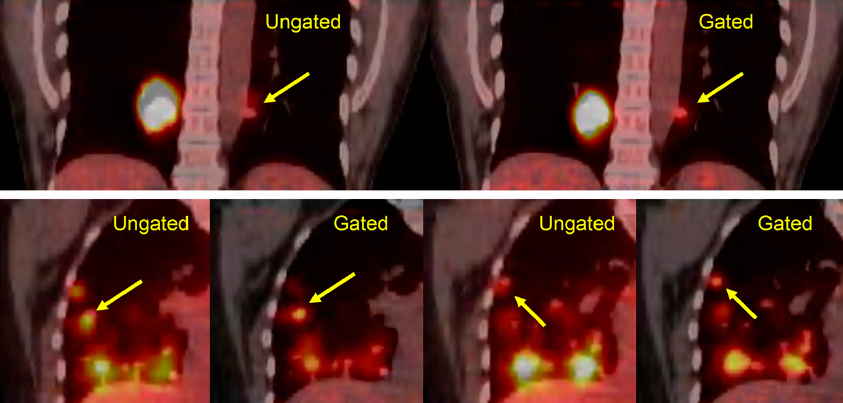
\includegraphics[width=10cm]{images/chang2010}
		\end{tabular}
	\end{center}
	\caption{Images TEP/TDM superposées du poumon reconstruites avec et sans gating respiratoire en utilisant la méthode décrite dans~\cite{GuopingChang2010Implementation}. On peut observer que les tumeurs sont mieux définies et correspondent à l'image TDM qui sert de référence.} 
	\label{fig:chang2010}
\end{figure}

Le principal problème de ces techniques est qu'elles demandent un temps d'acquisition beaucoup plus long à qualité d'image égale. Si l'on ne conserve que 20\% des évènements détectés, cela signifie qu'il faut augmenter le temps d'acquisition d'un facteur 5 pour obtenir une image d'une qualité égale. Il n'est donc pas envisageable de mettre en place ces protocoles en routine clinique, car le temps disponible n'est pas suffisant. C'est pour cela que de nombreuses équipes se sont mises à travailler sur une évolution de cette technique, où les images sont déformées les unes sur les autres pour prendre en compte toutes les informations de l'acquisition.

\section{Synchronisation respiratoire avec recalage}
\label{lab:corrPostRecon}

Dans cette section, nous allons détailler la technique consistant à corriger  le mouvement en déformant les images reconstruites.

Pour réaliser cela, les différentes techniques se basent sur une estimation préalable du mouvement respiratoire. Les images de chaque phase sont reconstruites indépendamment, puis recalées sur une phase de référence grâce au champ de mouvement. Enfin, les images déformées sont sommées. La difficulté se situe dans l'estimation du champ de mouvement interne lors de la respiration, car ce mouvement est complexe.

Les premières publications décrivant cette technique l'utilisaient notamment pour réaliser de l'imagerie cardiaque en TEP~\cite{klein19973d}. Cette publication démontre la faisabilité du procédé sur un animal en utilisant des techniques de flux optique pour estimer le champ de mouvement. En effet le coeur a l'avantage d'avoir une activité métabolique intense, ce qui rend l'estimation de son mouvement aisée même sur des images avec une faible statistique.

\subsection{Estimation du mouvement respiratoire corps entier}

L'estimation du champ de mouvement interne se fait à l'aide d'une des techniques présentées précédemment en \ref{lab:estimChamp}. Elles sont rappelées brièvement :

\subsubsection{imagerie TEP avec gating}
\label{lab:correctionDawood2008}

L`'acquisition TEP est réalisée en même temps que le signale respiratoire. Une image est reconstruite par phase du signal respiratoire, puis un algorithme d'estimation de mouvement est utilisé pour calculer le champ de mouvement entre les instants du cycle.

Les premiers algorithmes étaient utilisés en imagerie cardiaque~\cite{klein2002four} avec des transformations simples (affines), puis d'autres algorithmes plus adaptés aux images corps entier ont été utilisées, comme les flux optiques~\cite{dawood2006lung, dawood2006lung}, ou l'interpolation par B-spline~\cite{bai2009regularized}. 


\subsubsection{imagerie CT 4D}

Les images CT 4D peuvent être utilisées pour réaliser l'estimation du mouvement respiratoire au lieu des données TEP. Cela nécessite par contre une dose plus importante et un temps d'acquisition plus long.
Dawood a réalisé plusieurs publications sur le sujet en utilisant le flux optique pour l'estimation du champ de mouvement~\cite{dawood2006lung, dawood2008respiratory}. L'algorithme a été étudié sur des images de patients réels. Une autre publication~\cite{thorndyke2006reducing} indique une amélioration du rapport de contraste sur bruit (CNR) d'un facteur 3 grâce à la correction.


\section{Correction pré-reconstruction}

Les méthodes de correction du mouvement pré-reconstruction modifient les positions des Lignes de réponse (LDR) fournies par le scanner.
Ce recalage des LDR correspond à un déplacement des lignes de réponse dans l'espace du détecteur (voir fig. \ref{fig:recalageLOR}) en fonction du mouvement respiratoire. La limitation principale de ce type de méthode est que le champ de mouvement ne peut pas être élastique.

Cependant, il a été étudié en imagerie du cerveau~\cite{bloomfield2003design}, où il permettait de corriger les mouvements de la tête. Il a été aussi utilisé en imagerie cardiaque TEP~\cite{livieratos2005rigid} en utilisant un champ de mouvement rigide (rotation suivie d'une translation).

Dans les deux cas, les résultats ont montrés une nette amélioration des images (voir fig. \ref{fig:ameliorationLOR}

Dans le cadre du mouvement respiratoire du thorax, l'approche de recalage par LDR a été expérimentée par Frédéric Lamare~\cite{lamare2007respiratory}, mais avec des résultats mitigés.

\begin{figure}[h!]
	\begin{center}
		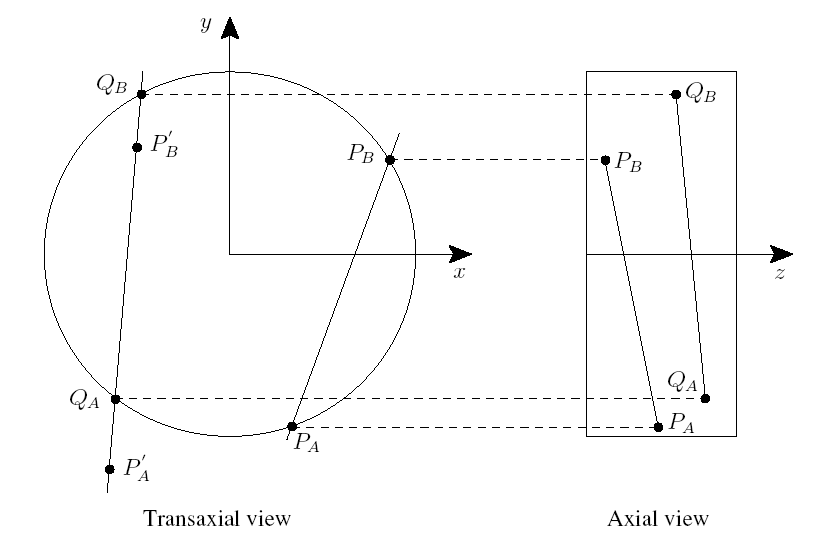
\includegraphics[width=12cm]{images/recalageLOR}
	\end{center}
	\caption{Illustration du recalage des lignes de réponse dans l'espace du détecteur : $P_A$ et $P_B$ représentent les positions des détections, $P_{A'}$ et $P_{B'}$ les positions des points corrigé et $Q_A$ et $Q_B$ les détections correspondantes } 
	\label{fig:recalageLOR}
\end{figure}

\begin{figure}[h!]
	\begin{center}
		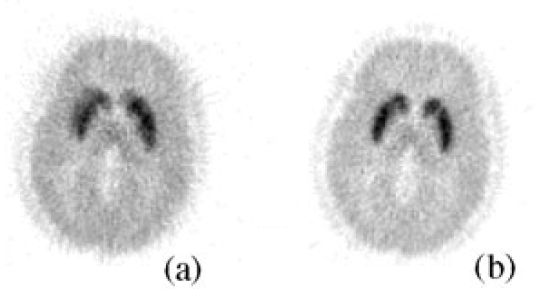
\includegraphics[width=6cm]{images/bloomfield2003design} 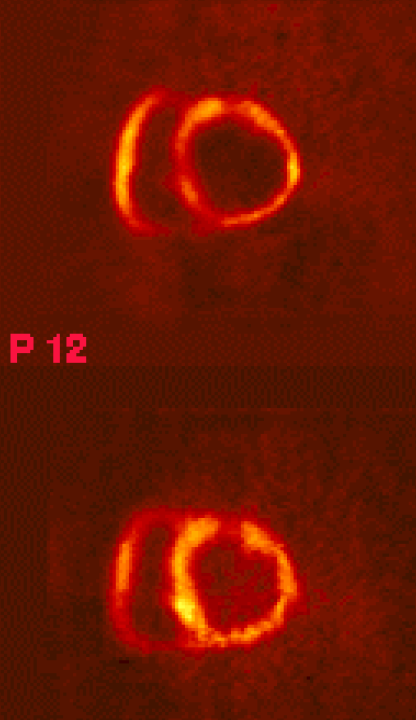
\includegraphics[width=3cm]{images/livieratos2005rigid}
	\end{center}
	\caption{Résultats de l'algorithme de recalage des LOR sur des images de patients utilisant le radio-traceur [$^{11}$C]raclopride. (a) montre une image non corrigée du mouvement et (b) une image corrigée. On peut noter que les éléments internes du cerveau sont beaucoup mieux définis. (c) représente une coupe du coeur petit axe non corrigée (en haut) et corrigée (en bas). On peut voir une amélioration de la définition de l'image.} 
	\label{fig:ameliorationLOR}
\end{figure}
 
Cette technique de correction du mouvement a été utilisée pour la correction du mouvement respiratoire du thorax~\cite{lamare2007respiratory,lamare2007list}, avec des performances plus limitées. En effet, le champ était approximé par une transformation affine, qui peut difficilement modéliser le mouvement du thorax dans son ensemble.

En effet, \cite{lamare2007respiratory} réalise une estimation du mouvement affine, en recalant les images TDM de chaque instant du cycle sur l'image de référence à l'aide d'une transformation affine par maximisation de l'information mutuelle normalisée. Le champ de mouvement  est calculé séparément pour le poumon, le coeur et trois organes sous le diaphragme (foie, estomac, rate). Les données sont des simulations réalisées par Geant4~\cite{jan2004gate} pour simuler un imageur Philips Allegro.

Ces résultats ont été améliorés par l'utilisation de la technique suivante qui permettait la prise en compte d'un mouvement élastique.

\section{Correction pendant la reconstruction}
\label{lab:CorrpendantRecon}
Plusieurs auteurs ont présentés des méthodes permettant de réaliser la correction de mouvement pendant la reconstruction. Qiao et al.\cite{qiao2006motion} et Lamare et al.~\cite{lamare2007list} ont proposé une méthode de correction du mouvement respiratoire basé sur une modification de la matrice de sensibilité lors de la reconstruction pour prendre en compte le mouvement. Tous les deux utilisent un champ de mouvement élastique estimé en utilisant un champ interpolé par B-splines.

L'algorithme original utilisé est basé sur OPL-EM~\cite{reader2002one} qui organise les données en ``sous-ensemble'' de la même manière que OS-EM~\cite{hudson1994accelerated} mais en utilisant les informations list-mode. Le principe de la reconstruction avec correction du mouvement respiratoire est décrit par la formule suivante :

\label{lab:corrMatSyst}
\begin{equation}
 f^{k+1}=\frac{f^k}{S} \sum_{t=1}^{N_{frames}} P_t^T \frac{1}{P_t f^k} 
\end{equation}

$f^k$ est l'image à l'itération $k$,

$T$ est l'opérateur de transposition

$P_t$ représente la matrice système à l'instant t. Chaque élément $p_{ij}$ de cette matrice indique la probabilité de détecter à la ligne de réponse $i$ un évènement généré au voxel $j$. 

$N$ correspond au nombre d'instants temporels considérés.

$S$ est la matrice de sensibilité :

\begin{equation}
 S=\frac{1}{N_{frames}} \sum_{t=1}^{N_{frames}} P_t^T N A_t 
\end{equation}

 $A_t$ est la matrice permettant de corriger les effets de l'atténuation au temps $t$ et $N$ est la matrice de normalisation qui compense l'inhomogénéité spatiale de la sensibilité.

Dans la publication~\cite{lamare2007list}, deux variantes de cette technique sont comparées avec la correction par synchronisation respiratoire avec recalage présentée précédemment ainsi que la correction pré-reconstruction. Les résultats présentés montrent un clair avantage pour la correction pendant la reconstruction, avec des performances couramment améliorées d'un facteur 2. 

Par exemple, la différence relative du contraste (équation \ref{eq:percentAmelioraiton}) pour une lésion de 7mm présente dans la partie haute du poumon est de 28\% pour les images non corrigées, contre 4.4\% pour les images corrigées par la méthode de correction pré-reconstruction et de 1.2\% pour la méthode de reconstruction pendant la reconstruction. De la même manière, pour des lésions de 7mm présentes dans le bas du poumon, les images non corrigées montrent une différence relative de contraste de 32\%, contre 2.63\% pour la correction pré-reconstruction et 1.66\% pour la correction pendant la reconstruction.


\begin{equation}
 \label{eq:percentAmelioraiton}
 \% Am\acute{e}lioration = \left| \frac{Image~\acute{E}valu\acute{e}e~-~R\acute{e}f\acute{e}rence}{R\acute{e}f\acute{e}rence} \right|
\end{equation}

La figure \ref{fig:lamare2007} montre un profil de l'interface poumon/foie avec une tumeur pour les différentes techniques de correction. On voit clairement que l'image non corrigée montre un retard dû au flou de mouvement. Ce retard est partiellement corrigé par la correction de mouvement pré-reconstruction, mais le profil de courbe de la méthode de correction du mouvement pendant la reconstruction est celui qui s'approche le plus de la référence.


\begin{figure}[h!]
	\begin{center}
		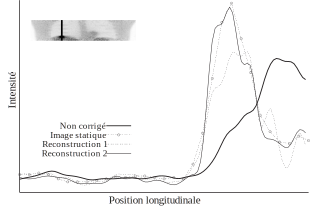
\includegraphics[width=12cm]{images/lamare2007list}
	\end{center}
	\caption{comparaison des performances des différentes techniques de correction du mouvement sur un profil d'image TEP contenant une tumeur placée au niveau du diaphragme. La référence correspond à Frame 1, LORs-Affine correspond à la correction pré-reconstruction et Elastic Method 2 corresponds à la correction pendant la reconstruction.} 
	\label{fig:lamare2007}
\end{figure}


\section{Déconvolution de l'image}

Cette technique décrite en ~\cite{naqa2006deblurring} utilise une connaissance du mouvement respiratoire acquise à partir d'une image TDM 4D pour déduire un filtrage appelé TLP (\textit{Tumor Location Probability}) qui correspond à la dégradation dû au mouvement respiratoire.

L'image est ensuite déconvoluée pour corriger les effets du mouvement respiratoire. Cette méthode a été évaluée sur un fantôme physique et des patients réels à l'aide d'un grand nombre de critères provenant pour partie de la TEP (sous-estimation de l'activité de la tumeur, exemples d'images), et pour partie du domaine de la déconvolution (entropie, ``rugosité'').

Les résultats présentés en \ref{fig:performanceDeconvolution} montrent une nette amélioration des performances sur des fantômes, pour un déplacement axial simple de 20mm. L'activité des lésions de fort diamètre est correctement récupérée quelque soit l'algorithme utilisée, mais il n'a pratiquement pas d'effets sur les lésions de 1cm de diamètre.

Ce type d'algorithme est peu présenté dans la littérature. 

\begin{figure}[h!]
	\begin{center}
		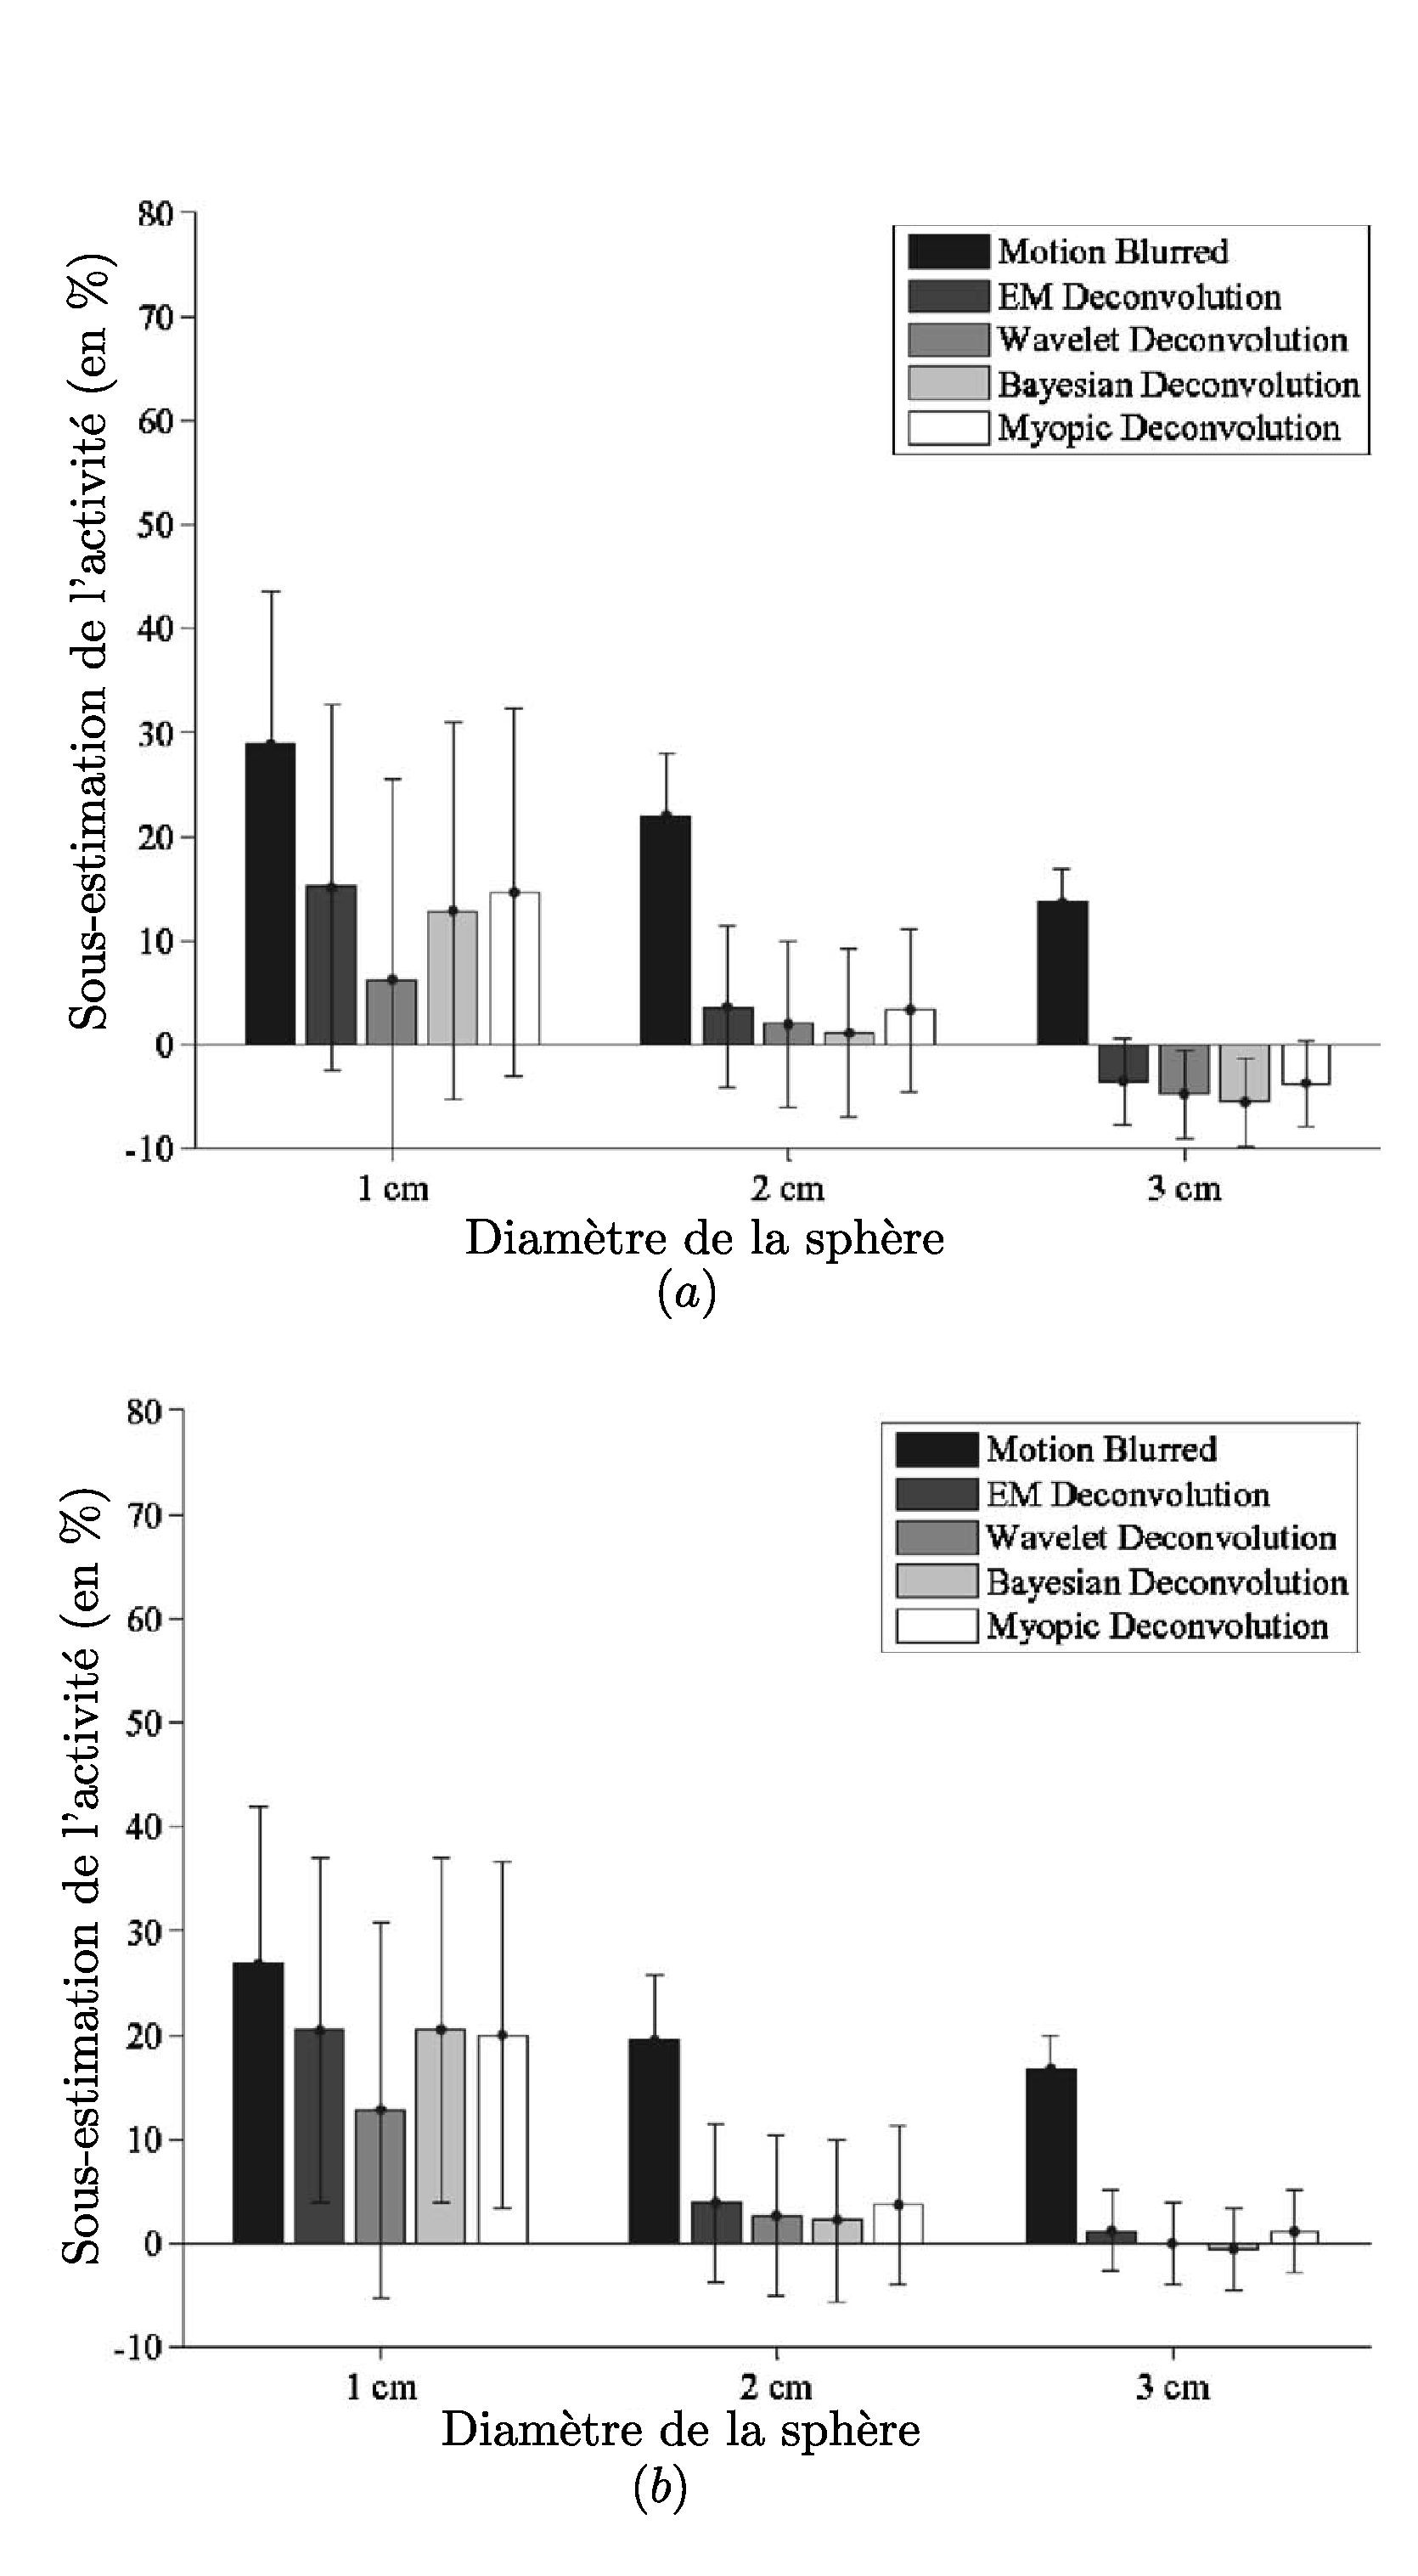
\includegraphics[width=10cm]{images/performanceDeconvolution}
	\end{center}
	\caption{Comparaison de l'erreur de sous-estimation de l'activité des lésions en fonction de l'algorithme de déconvolution utilisé sur des fantômes. En a) la lésion a une activité moyenne, tandis qu'en b) l'activité de la lésion est faible par rapport au fond. Le déplacement de la lésion est le même dans les deux cas (2cm)} 
	\label{fig:performanceDeconvolution}
\end{figure}


Un autre article utilisant aussi des algorithmes de déconvolution a été présenté par wiemker~\cite{wiemker2008combined}. Cependant il ne cherche pas à corriger le mouvement respiratoire sur l'ensemble de l'image mais principalement à améliorer la mesure du SUV sur une lésion. Pour cela, il réalise une estimation de la fonction d'étalement du point (FEP) de l'imageur TEP au niveau de la lésion à l'aide d'un contourage de la lésion réalisé préalablement dur une image TDM. L'estimation de la FEP permet de prendre en compte à la fois les effets du mouvement respiratoire et ceux de la FEP intrinsèque à l'imageur TEP. 

Cependant, cette technique est inapplicable dans notre cas car les lésions doivent être suffisamment importantes et homogènes pour pouvoir les délimiter de manière fiable sur les images TDM, ce qui n'est pas notre cas.
